\documentclass[12pt]{article}
\usepackage{amsmath}
\usepackage{times}
\usepackage{anyfontsize}
\usepackage{amsfonts}
\usepackage[paperheight=12in,paperwidth=12in,margin=1in]{geometry}
\usepackage{tikz}
%\usepackage[x11names]{xcolor}
\usepackage{tcolorbox}

\usepackage{graphicx}
\graphicspath{{images/}}
\begin{document}
	
\newtcolorbox{mybox}{colback=blue!5!white,colframe=blue}
\begin{tikzpicture}[remember picture,overlay]
\coordinate [below=12cm] (midpoint) at (current page.north);
\node at (current page.north west)
{\begin{tikzpicture}[remember picture,overlay]
	\node[anchor=north west,inner sep=0pt,opacity=0.2] at (0,0) {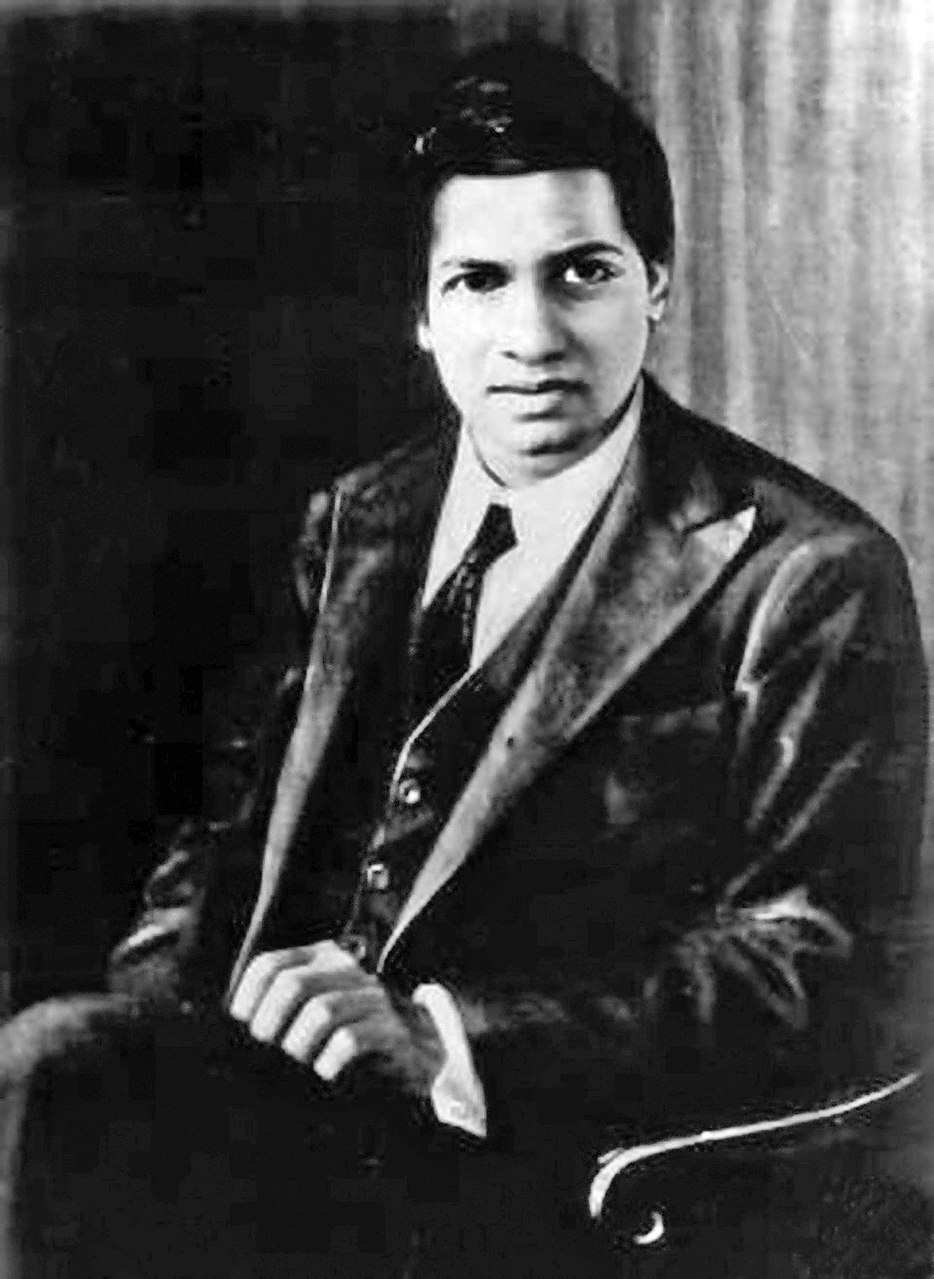
\includegraphics[width=\paperwidth]{2.jpg}}; % Background image
	\end{tikzpicture}};
\end{tikzpicture}
\color{blue}
	\begin{center}
		\thispagestyle{empty}
		%\pagecolor{BrickRed}
		\color{blue}
		
		{\fontsize{40}{20}\selectfont\textbf{\underline{Functional Equation Week: Problem 5}}}
		
		\vspace*{1cm}
		
		{\fontsize{35}{30}\selectfont\textbf{Send me Your Answer!}}
		\vspace*{1cm}
	\end{center}
		
		{\fontsize{30}{30}\selectfont Find all functions $ f : \mathbb R\to \mathbb R$ such that \[ x^2y^2 \left( f(x+y)-f(x)-f(y) \right)=3(x+y)f(x)f(y)\] holds for all reals $x$ and $y$}
		
		\vspace{1cm}
	\begin{center}	
		{\fontsize{30}{30}\textbf{ONLY ELEMENTARY SOLUTIONS ALLOWED}}
		
		\vspace{1cm}

{\fontsize{50}{60}\selectfont 
		
		$$\boldsymbol{\sum \limits_{i=0}^{Creative} Math_i = Solving}$$}
		
		\vspace{1cm}
		
		\begin{mybox}\Huge{\begin{center}\textbf{\textcolor{blue}{Solution $\to$}} \end{center}}\end{mybox}
	\end{center}
\end{document}